% Options for packages loaded elsewhere
% Options for packages loaded elsewhere
\PassOptionsToPackage{unicode}{hyperref}
\PassOptionsToPackage{hyphens}{url}
%
\documentclass[
  ignorenonframetext,
  aspectratio=169,
]{beamer}
\newif\ifbibliography
\usepackage{pgfpages}
\setbeamertemplate{caption}[numbered]
\setbeamertemplate{caption label separator}{: }
\setbeamercolor{caption name}{fg=normal text.fg}
\beamertemplatenavigationsymbolsempty
% remove section numbering
\setbeamertemplate{part page}{
  \centering
  \begin{beamercolorbox}[sep=16pt,center]{part title}
    \usebeamerfont{part title}\insertpart\par
  \end{beamercolorbox}
}
\setbeamertemplate{section page}{
  \centering
  \begin{beamercolorbox}[sep=12pt,center]{section title}
    \usebeamerfont{section title}\insertsection\par
  \end{beamercolorbox}
}
\setbeamertemplate{subsection page}{
  \centering
  \begin{beamercolorbox}[sep=8pt,center]{subsection title}
    \usebeamerfont{subsection title}\insertsubsection\par
  \end{beamercolorbox}
}
% Prevent slide breaks in the middle of a paragraph
\widowpenalties 1 10000
\raggedbottom
\usepackage{iftex}
\ifPDFTeX
  \usepackage[T1]{fontenc}
  \usepackage[utf8]{inputenc}
  \usepackage{textcomp} % provide euro and other symbols
\else % if luatex or xetex
  \usepackage{unicode-math} % this also loads fontspec
  \defaultfontfeatures{Scale=MatchLowercase}
  \defaultfontfeatures[\rmfamily]{Ligatures=TeX,Scale=1}
\fi
\usepackage{lmodern}

\usetheme[]{metropolis}
\ifPDFTeX\else
  % xetex/luatex font selection
\fi
% Use upquote if available, for straight quotes in verbatim environments
\IfFileExists{upquote.sty}{\usepackage{upquote}}{}
\IfFileExists{microtype.sty}{% use microtype if available
  \usepackage[]{microtype}
  \UseMicrotypeSet[protrusion]{basicmath} % disable protrusion for tt fonts
}{}
\makeatletter
\@ifundefined{KOMAClassName}{% if non-KOMA class
  \IfFileExists{parskip.sty}{%
    \usepackage{parskip}
  }{% else
    \setlength{\parindent}{0pt}
    \setlength{\parskip}{6pt plus 2pt minus 1pt}}
}{% if KOMA class
  \KOMAoptions{parskip=half}}
\makeatother


\usepackage{longtable,booktabs,array}
\usepackage{calc} % for calculating minipage widths
\usepackage{caption}
% Make caption package work with longtable
\makeatletter
\def\fnum@table{\tablename~\thetable}
\makeatother
\usepackage{graphicx}
\makeatletter
\newsavebox\pandoc@box
\newcommand*\pandocbounded[1]{% scales image to fit in text height/width
  \sbox\pandoc@box{#1}%
  \Gscale@div\@tempa{\textheight}{\dimexpr\ht\pandoc@box+\dp\pandoc@box\relax}%
  \Gscale@div\@tempb{\linewidth}{\wd\pandoc@box}%
  \ifdim\@tempb\p@<\@tempa\p@\let\@tempa\@tempb\fi% select the smaller of both
  \ifdim\@tempa\p@<\p@\scalebox{\@tempa}{\usebox\pandoc@box}%
  \else\usebox{\pandoc@box}%
  \fi%
}
% Set default figure placement to htbp
\def\fps@figure{htbp}
\makeatother





\setlength{\emergencystretch}{3em} % prevent overfull lines

\providecommand{\tightlist}{%
  \setlength{\itemsep}{0pt}\setlength{\parskip}{0pt}}



 


% ============================================================
%  Econ 2203 — Beamer Metropolis Theme Preamble
%  Course: International Trade and Policy in Agriculture
%  Instructor: Nithin M, Department of Development Economics
% ============================================================

% MUST be first: load Metropolis theme before \metroset and colour overrides
\usetheme{metropolis}

% Only load packages not already provided by pandoc's beamer template
\usepackage{amsmath,amssymb}

% ---- Brand colours -----------------------------------------
\definecolor{brandblue}{HTML}{012169}
\definecolor{brandgold}{HTML}{B9975B}
\definecolor{lightblue}{HTML}{E8EDF5}

% ---- Metropolis colour overrides ---------------------------
% Main palette
\setbeamercolor{normal text}{fg=black,bg=white}
\setbeamercolor{background canvas}{bg=white}
\setbeamercolor{alerted text}{fg=brandgold}
\setbeamercolor{example text}{fg=brandblue!70!black}

% Title slide
\setbeamercolor{title}{fg=white,bg=brandblue}
\setbeamercolor{subtitle}{fg=brandgold}
\setbeamercolor{author}{fg=white}
\setbeamercolor{institute}{fg=brandgold!80!white}
\setbeamercolor{date}{fg=white}
\setbeamercolor{title page header}{fg=white,bg=brandblue}

% Frametitle bar
\setbeamercolor{frametitle}{fg=white,bg=brandblue}

% Progress bar → gold
\setbeamercolor{progress bar}{fg=brandgold,bg=brandblue!30}
\setbeamercolor{title separator}{fg=brandgold}
\setbeamercolor{progress bar in head/foot}{fg=brandgold,bg=brandblue!20}
\setbeamercolor{progress bar in section page}{fg=brandgold,bg=brandblue!20}

% Blocks
\setbeamercolor{block title}{bg=brandblue,fg=white}
\setbeamercolor{block body}{bg=lightblue,fg=black}
\setbeamercolor{block title alerted}{bg=brandgold,fg=white}
\setbeamercolor{block body alerted}{bg=brandgold!12,fg=black}
\setbeamercolor{block title example}{bg=brandblue!70!black,fg=white}
\setbeamercolor{block body example}{bg=brandblue!8,fg=black}

% Structure / lists
\setbeamercolor{structure}{fg=brandblue}
\setbeamercolor{section in toc}{fg=brandblue}
\setbeamercolor{itemize item}{fg=brandblue}
\setbeamercolor{itemize subitem}{fg=brandgold}
\setbeamercolor{enumerate item}{fg=brandblue}
\setbeamercolor{description item}{fg=brandblue}

% ---- Metropolis options ------------------------------------
\metroset{
  progressbar    = frametitle,   % gold bar under frametitle
  sectionpage    = none,
  numbering      = fraction,
  block          = fill
}

% ---- Fonts (Metropolis uses Fira Sans; fallback gracefully) -
\setbeamerfont{title}{size=\Large,series=\bfseries}
\setbeamerfont{subtitle}{size=\normalsize,series=\mdseries}
\setbeamerfont{frametitle}{size=\large,series=\bfseries}
\setbeamerfont{block title}{size=\normalsize,series=\bfseries}
\setbeamerfont{caption}{size=\footnotesize}

% ---- Footer: lecture title + course + slide number ----------
\setbeamertemplate{footline}{%
  \begin{beamercolorbox}[wd=\paperwidth,ht=2.0ex,dp=1ex]{footline}%
    \hspace{0.8em}%
    {\footnotesize\color{brandblue!60}%
      \insertshorttitle
      \hfill Nithin M \hfill
      \insertframenumber{}/\inserttotalframenumber\hspace{0.8em}}%
  \end{beamercolorbox}%
}

% ---- Misc --------------------------------------------------
\setlength{\parskip}{2pt}
\setbeamertemplate{navigation symbols}{}

% tighter column sep for side-by-side content
\setlength{\columnsep}{0.8em}

% ---- Max 6 lines per slide: compact list typesetting -------
% Smaller fonts at each list depth
\setbeamerfont{itemize/enumerate body}{size=\small}
\setbeamerfont{itemize/enumerate subbody}{size=\footnotesize}
\setbeamerfont{itemize/enumerate subsubbody}{size=\scriptsize}

% Tight vertical spacing injected at the start of each list level
\setbeamertemplate{itemize/enumerate body begin}{%
  \setlength{\itemsep}{3pt}\setlength{\parsep}{0pt}}
\setbeamertemplate{itemize/enumerate subbody begin}{%
  \setlength{\itemsep}{2pt}\setlength{\parsep}{0pt}}
\setbeamertemplate{itemize/enumerate subsubbody begin}{%
  \setlength{\itemsep}{1pt}\setlength{\parsep}{0pt}}

% Global safety net: default frame shrink = 10 %
% \beamer@shrinkfalse is called ONCE in beamer's frame init (line 438 of
% beamerbaseframe.sty) before the user's options are processed (line 444).
% By redefining it we inject shrink=10 right after the reset; if the frame
% explicitly specifies [shrink=X], the later \setkeys call overrides it.
\makeatletter
\let\beamer@orig@shrinkfalse\beamer@shrinkfalse
\def\beamer@shrinkfalse{%
  \beamer@orig@shrinkfalse
  \setkeys{beamerframe}{shrink=10}}
\makeatother

% Fix: make \label truly robust in moving arguments.
% Quarto wraps figure labels inside captions; Metropolis expands them
% in batchmode causing a crash. DeclareRobustCommand prevents expansion.
\makeatletter
\let\quarto@originallabel\label
\DeclareRobustCommand*{\label}[1]{\quarto@originallabel{#1}}
\makeatother

% Prevent figures from overflowing Beamer frames.
% width=\linewidth: scale to text width (already Quarto default);
% height=0.6\textheight: cap height so figures never push past the frame bottom.
% keepaspectratio: never distort — whichever constraint binds first wins.
\setkeys{Gin}{width=\linewidth,height=0.55\textheight,keepaspectratio}
\makeatletter
\@ifpackageloaded{caption}{}{\usepackage{caption}}
\AtBeginDocument{%
\ifdefined\contentsname
  \renewcommand*\contentsname{Table of contents}
\else
  \newcommand\contentsname{Table of contents}
\fi
\ifdefined\listfigurename
  \renewcommand*\listfigurename{List of Figures}
\else
  \newcommand\listfigurename{List of Figures}
\fi
\ifdefined\listtablename
  \renewcommand*\listtablename{List of Tables}
\else
  \newcommand\listtablename{List of Tables}
\fi
\ifdefined\figurename
  \renewcommand*\figurename{Figure}
\else
  \newcommand\figurename{Figure}
\fi
\ifdefined\tablename
  \renewcommand*\tablename{Table}
\else
  \newcommand\tablename{Table}
\fi
}
\@ifpackageloaded{float}{}{\usepackage{float}}
\floatstyle{ruled}
\@ifundefined{c@chapter}{\newfloat{codelisting}{h}{lop}}{\newfloat{codelisting}{h}{lop}[chapter]}
\floatname{codelisting}{Listing}
\newcommand*\listoflistings{\listof{codelisting}{List of Listings}}
\makeatother
\makeatletter
\makeatother
\makeatletter
\@ifpackageloaded{caption}{}{\usepackage{caption}}
\@ifpackageloaded{subcaption}{}{\usepackage{subcaption}}
\makeatother

\usepackage{bookmark}
\IfFileExists{xurl.sty}{\usepackage{xurl}}{} % add URL line breaks if available
\urlstyle{same}
\hypersetup{
  pdftitle={Lecture 9: Balance of Trade \& Balance of Payments},
  pdfauthor={Nithin M},
  hidelinks,
  pdfcreator={LaTeX via pandoc}}


\title[L9 \textbar{} Balance of Trade \& Payments]{Lecture 9: Balance of
Trade \& Balance of Payments}
\subtitle{Econ 2203 \textbar{} International Trade and Policy in
Agriculture}
\author{Nithin M}
\date{2026-06-20}
\institute{Department of Development Economics}

\begin{document}
\frame{\titlepage}


\begin{frame}{Introduction: Why the BoP Matters}
\phantomsection\label{introduction-why-the-bop-matters}
\textbf{Key questions for today:}

\begin{itemize}
\tightlist
\item
  How does a country ``pay'' for its imports?
\item
  What happens when a country consistently imports more than it exports?
\item
  How do capital flows balance the external accounts?
\item
  When does a BoP \emph{crisis} occur?
\end{itemize}

\textbf{BoP accounting identity:}

\[\underbrace{\text{CA}}_{\text{trade + income}} + \underbrace{\text{KA}}_{\text{transfers}} + \underbrace{\text{FA}}_{\text{capital flows}} + \underbrace{\Delta R}_{\text{reserve change}} = 0\]

A current account deficit \emph{must} be financed by capital/financial
inflows or by running down foreign exchange reserves. If neither is
available → \textbf{BoP crisis} (India 1991).

\note{\textbf{India's external sector at a glance (FY2024):}

\begin{itemize}
\tightlist
\item
  Merchandise exports: \textbf{\$437 billion} (goods)
\item
  Merchandise imports: \textbf{\$677 billion} (goods)
\item
  Trade deficit: \textbf{-\$240 billion} (goods only)
\item
  Services surplus: \textbf{+\$163B}
\item
  Remittances: \textbf{+\$120B} (world's largest recipient)
\item
  Current account: \textbf{-\$23B (-0.7\% of GDP)}
\end{itemize}}
\end{frame}

\begin{frame}{Balance of Trade (BoT): the idea}
\phantomsection\label{balance-of-trade-bot-the-idea}
\[\text{BoT} = X_{goods} - M_{goods}\]

\begin{itemize}
\tightlist
\item
  BoT \textgreater{} 0: trade surplus
\item
  BoT \textless{} 0: trade deficit
\item
  India typically has a \textbf{goods deficit} (oil + gold +
  electronics)
\end{itemize}
\end{frame}

\begin{frame}{India FY2024: why the goods deficit persists}
\phantomsection\label{india-fy2024-why-the-goods-deficit-persists}
\begin{itemize}
\tightlist
\item
  Goods exports ≈ \textbf{\$437B}
\item
  Goods imports ≈ \textbf{\$677B}
\item
  Goods trade balance ≈ \textbf{-\$240B}
\end{itemize}

Structural drivers: crude oil dependence + gold demand + electronics
import intensity.
\end{frame}

\begin{frame}{Current Account identity (absorption approach)}
\phantomsection\label{current-account-identity-absorption-approach}
\[Y = C + I + G + (X - M)\]

Rearrange:

\[\boxed{\text{CA} \approx (X-M) = Y - A}\quad\text{where }A=C+I+G\]

\begin{itemize}
\tightlist
\item
  If \textbf{\(Y>A\)}: produce more than spend → net lender
\item
  If \textbf{\(Y<A\)}: spend more than produce → net borrower
\end{itemize}
\end{frame}

\begin{frame}{Current Account identity (saving--investment form)}
\phantomsection\label{current-account-identity-savinginvestment-form}
\[\boxed{\text{CA} = (S - I) + (T - G)}\]

\begin{itemize}
\tightlist
\item
  CA deficit can reflect \textbf{high investment} (good) or
  \textbf{fiscal deficit} (risk)
\item
  Devaluation alone won't fix CA if absorption stays high
\end{itemize}
\end{frame}

\begin{frame}{India FY2024: why the CA deficit was small}
\phantomsection\label{india-fy2024-why-the-ca-deficit-was-small}
\begin{itemize}
\tightlist
\item
  Goods trade deficit was large (≈ \textbf{-\$240B})
\item
  Services trade surplus was large (≈ \textbf{+\$163B})
\item
  Remittances were huge (≈ \textbf{+\$120B})
\item
  Net result: CA ≈ \textbf{-\$23B (-0.7\% of GDP)}
\end{itemize}

In India, services + remittances are the ``cushion'' behind the external
sector.
\end{frame}

\begin{frame}{BoP accounts: Current vs Capital}
\phantomsection\label{bop-accounts-current-vs-capital}
\begin{itemize}
\tightlist
\item
  \textbf{Current Account (CA):} goods, services, income, transfers
\item
  \textbf{Capital Account (KA):} capital transfers (usually small)
\item
  \textbf{Financial Account (FA):} FDI, FPI, loans, deposits, reserves
\end{itemize}
\end{frame}

\begin{frame}{Double-entry bookkeeping (2 examples)}
\phantomsection\label{double-entry-bookkeeping-2-examples}
\begin{itemize}
\tightlist
\item
  Import machines worth \$10M: CA \textbf{-10} and FA \textbf{+10}
\item
  Export software worth \$5M: CA \textbf{+5} and FA \textbf{-5} (forex
  asset)
\end{itemize}

Every transaction has equal-and-opposite entries → accounts always add
up.
\end{frame}

\begin{frame}{Financial Account and BoP Identity}
\phantomsection\label{financial-account-and-bop-identity}
\end{frame}

\begin{frame}{The Balance of Payments (BoP): Accounts + Identity}
\phantomsection\label{the-balance-of-payments-bop-accounts-identity}
\begin{itemize}
\tightlist
\item
  \textbf{Current Account (CA):} goods, services, income, transfers
\item
  \textbf{Capital Account (KA):} capital transfers (typically small)
\item
  \textbf{Financial Account (FA):} FDI, FPI, loans, and reserve changes
\item
  \textbf{Accounting identity:}
  \(\text{CA} + \text{KA} + \text{FA} + \Delta R = 0\)
\item
  If a CA deficit cannot be financed → \textbf{BoP crisis} (India 1991)
\end{itemize}
\end{frame}

\begin{frame}{India: BoP snapshot (FY2024)}
\phantomsection\label{india-bop-snapshot-fy2024}
\begin{longtable}[]{@{}ll@{}}
\toprule\noalign{}
Component & USD B \\
\midrule\noalign{}
\endhead
Current Account & -23 \\
Financial Account & +20 \\
Δ Reserves & +3 \\
\textbf{Total} & \textbf{≈ 0} \\
\bottomrule\noalign{}
\end{longtable}

\note{The CA deficit is financed primarily through FDI and portfolio
inflows, making FA stability critical.}
\end{frame}

\begin{frame}{India's BoP Components: FY2020--FY2024}
\phantomsection\label{indias-bop-components-fy2020fy2024}
\begin{figure}

\centering{

\pandocbounded{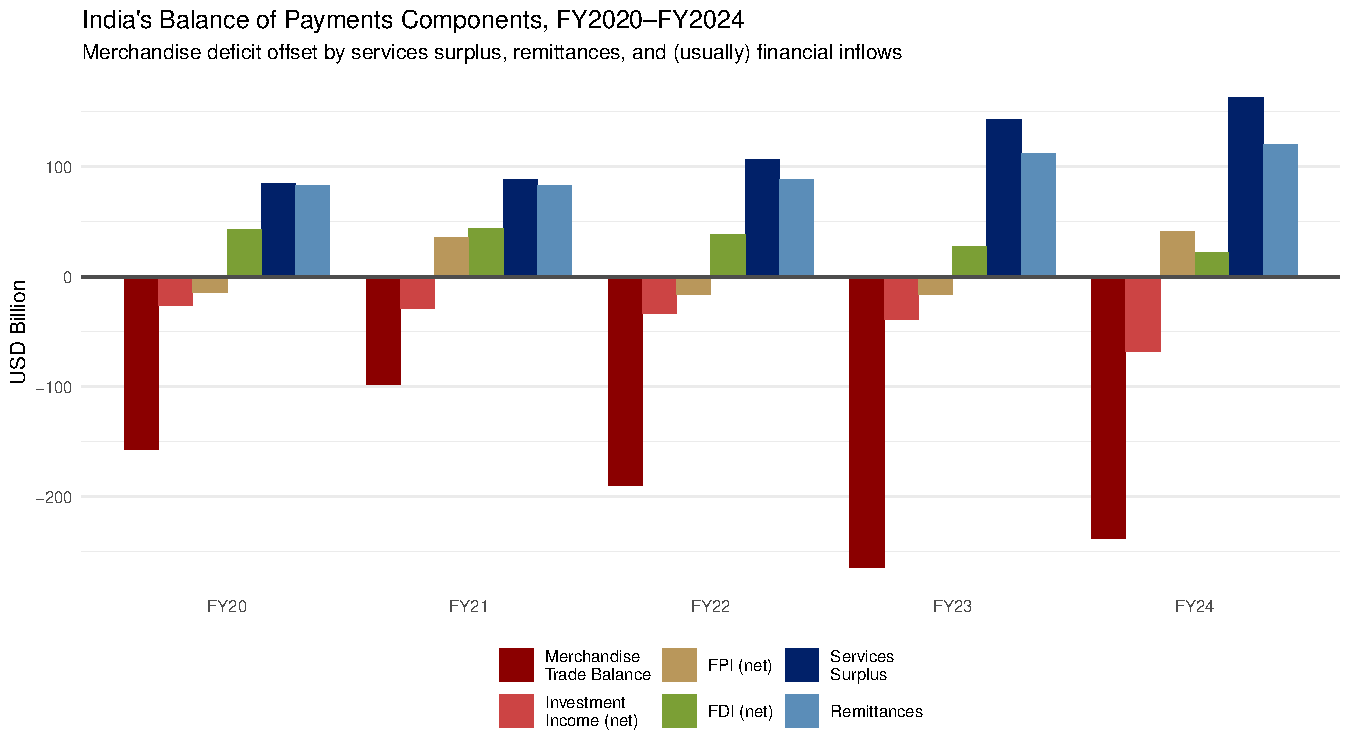
\includegraphics[keepaspectratio]{Lecture09_BoT_BoP_files/figure-beamer/fig-bop-india-1.pdf}}

}

\caption{India's Balance of Payments Components,
FY2020--FY2024 (USD billion) Source: RBI, Balance of Payments
Statistics.}
\label{fig-bop-india}

\end{figure}%
\end{frame}

\begin{frame}{India's Current Account: FY2024 Decomposition}
\phantomsection\label{indias-current-account-fy2024-decomposition}
\begin{figure}

\centering{

\pandocbounded{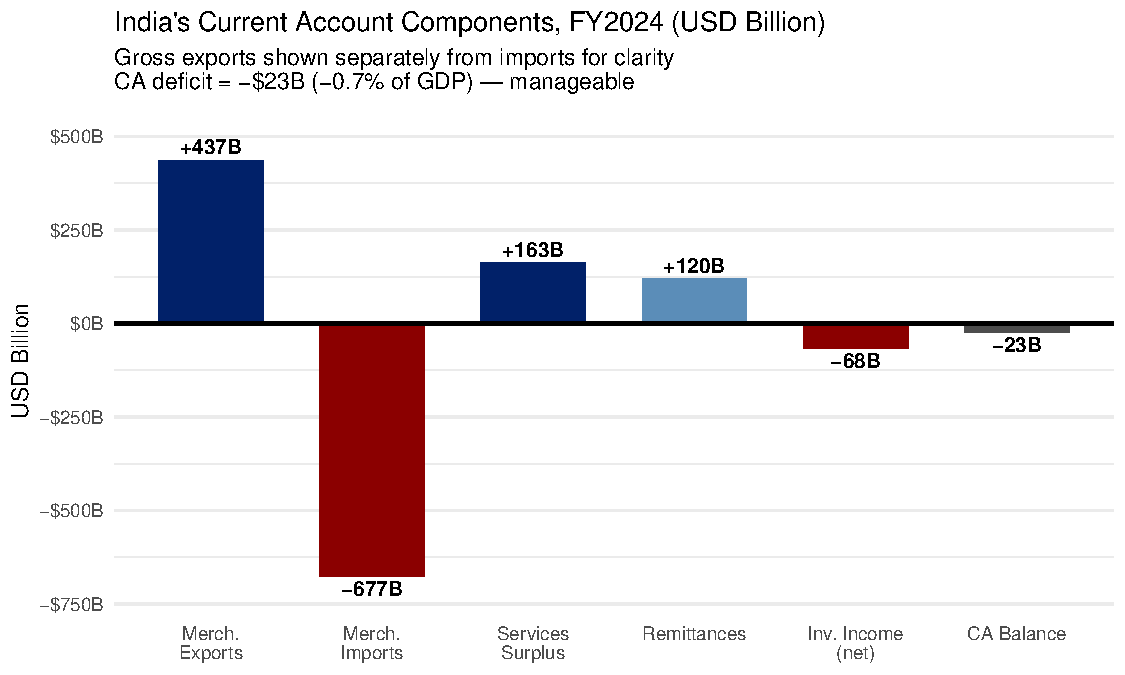
\includegraphics[keepaspectratio]{Lecture09_BoT_BoP_files/figure-beamer/fig-ca-waterfall-1.pdf}}

}

\caption{India's Current Account, FY2024:
Component Contributions (USD Billion) Source: RBI, Balance of Payments
Statistics.}
\label{fig-ca-waterfall}

\end{figure}%
\end{frame}

\begin{frame}{Financial Account (FA): India FY2024 (headline)}
\phantomsection\label{financial-account-fa-india-fy2024-headline}
\begin{itemize}
\tightlist
\item
  FA inflows were positive (FDI + portfolio + loans + deposits)
\item
  This helped finance the CA deficit and support reserves
\end{itemize}

\[\text{BoP identity: } CA + KA + FA + \Delta R = 0\]
\end{frame}

\begin{frame}{FDI vs FPI (why it matters)}
\phantomsection\label{fdi-vs-fpi-why-it-matters}
\begin{itemize}
\tightlist
\item
  \textbf{FDI:} long-term ownership, more stable
\item
  \textbf{FPI:} liquid ``hot money'', more volatile
\item
  BoP vulnerability often comes from \textbf{sudden stops} in
  FPI/short-term flows
\end{itemize}
\end{frame}

\begin{frame}{Forex reserves: what they are}
\phantomsection\label{forex-reserves-what-they-are}
\begin{itemize}
\tightlist
\item
  Foreign currency assets (USD/EUR/GBP/JPY, etc.)
\item
  Gold
\item
  SDRs + IMF reserve tranche
\item
  Used for liquidity in crises and to smooth extreme volatility
\end{itemize}

A common adequacy benchmark is ``months of import cover''.
\end{frame}

\begin{frame}{RBI intervention under a managed float}
\phantomsection\label{rbi-intervention-under-a-managed-float}
\begin{itemize}
\tightlist
\item
  \textbf{Buy USD / sell INR} to resist sharp appreciation
\item
  \textbf{Sell USD / buy INR} to resist sharp depreciation
\item
  Goal is usually to \textbf{smooth volatility}, not to fix a peg
\item
  Intervention affects reserves and domestic liquidity
\end{itemize}
\end{frame}

\begin{frame}{BoP adjustment mechanisms (3 channels)}
\phantomsection\label{bop-adjustment-mechanisms-3-channels}
\begin{itemize}
\tightlist
\item
  \textbf{Price (exchange rate):} depreciation switches demand toward
  domestic goods
\item
  \textbf{Income/absorption:} lower spending reduces imports
\item
  \textbf{Monetary/financial:} reserve loss tightens liquidity; rates
  rise; capital flows respond
\end{itemize}
\end{frame}

\begin{frame}{Typical policy instruments}
\phantomsection\label{typical-policy-instruments}
\begin{itemize}
\tightlist
\item
  \textbf{Devaluation / depreciation} (expenditure-switching)
\item
  \textbf{Fiscal/monetary tightening} (expenditure-reducing)
\item
  \textbf{Interest rate policy} to stabilise capital flows
\item
  \textbf{IMF financing} in reserve crises
\end{itemize}

India 1991 used a mix: devaluation + tightening + reforms.
\end{frame}

\begin{frame}{Marshall--Lerner condition}
\phantomsection\label{marshalllerner-condition}
\[\boxed{|e_X| + |e_M| > 1}\]

\begin{itemize}
\tightlist
\item
  Depreciation makes exports cheaper and imports costlier
\item
  Trade balance improves only if \textbf{quantities respond enough}
\item
  Short run: contracts + habits → weak quantity response
\end{itemize}
\end{frame}

\begin{frame}{Elasticities: short run vs long run}
\phantomsection\label{elasticities-short-run-vs-long-run}
\begin{itemize}
\tightlist
\item
  \textbf{Long run:} \(|e_X|\) and \(|e_M|\) tend to be higher → M--L
  more likely to hold
\item
  \textbf{Short run:} elasticities are low → trade balance can worsen
  first
\end{itemize}

This is the logic behind the J-curve.
\end{frame}

\begin{frame}{The J-Curve Effect}
\phantomsection\label{the-j-curve-effect}
\begin{figure}

\centering{

\pandocbounded{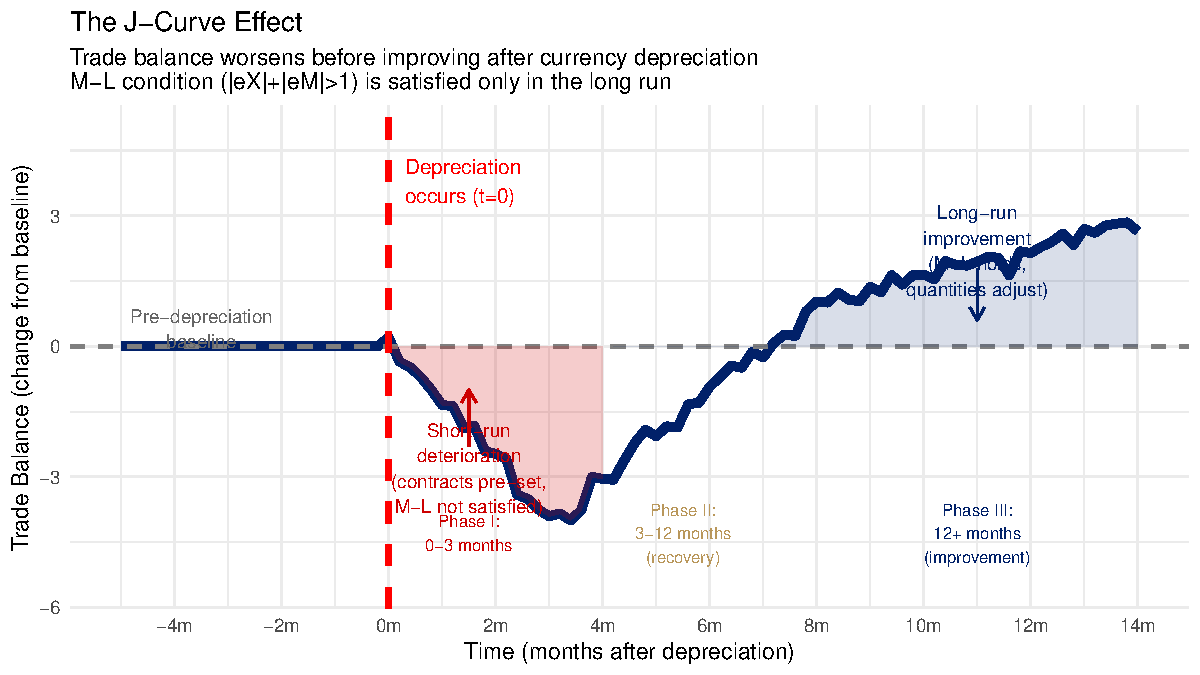
\includegraphics[keepaspectratio]{Lecture09_BoT_BoP_files/figure-beamer/fig-jcurve-1.pdf}}

}

\caption{J-Curve: Trade Balance Initially Worsens
After Currency Depreciation Source: Author's illustration.}
\label{fig-jcurve}

\end{figure}%
\end{frame}

\begin{frame}{J-curve: mechanisms (3 phases)}
\phantomsection\label{j-curve-mechanisms-3-phases}
\begin{itemize}
\tightlist
\item
  \textbf{Phase I (0--3 months):} contracts fixed → values move before
  quantities
\item
  Import bill can rise even if volumes don't
\item
  \textbf{Phase II (3--12 months):} firms adjust sourcing and sales
\item
  \textbf{Phase III (12+ months):} quantities respond fully
\item
  Long run: M--L more likely to hold → TB improves
\end{itemize}
\end{frame}

\begin{frame}{India: what we see in practice}
\phantomsection\label{india-what-we-see-in-practice}
\begin{itemize}
\tightlist
\item
  1991: large devaluation; adjustment took time (rigidities)
\item
  2013: TB improved faster as trade was more integrated
\item
  2022: oil prices dominated → weaker TB response
\item
  Agriculture adjusts faster than many manufactured goods (more spot
  pricing)
\end{itemize}
\end{frame}

\begin{frame}{Absorption approach: policy implication}
\phantomsection\label{absorption-approach-policy-implication}
\[\boxed{CA = Y - A}\quad (A=C+I+G)\]

\begin{itemize}
\tightlist
\item
  Improve CA by \textbf{raising output} (\(Y\)) and/or \textbf{reducing
  absorption} (\(A\))
\item
  Devaluation helps only if it changes quantities and spending patterns
\item
  Inflation can offset gains if real absorption doesn't fall
\end{itemize}
\end{frame}

\begin{frame}{India 1991: adjustment mix}
\phantomsection\label{india-1991-adjustment-mix}
\begin{itemize}
\tightlist
\item
  Fiscal tightening reduced absorption (\(\Delta G<0\))
\item
  Large devaluation switched demand toward domestic goods
\item
  Reforms improved long-run output capacity
\item
  CA improved over time, but growth fell temporarily
\item
  Inflation spiked during adjustment
\end{itemize}
\end{frame}

\begin{frame}{India's 1991 BoP crisis: what happened}
\phantomsection\label{indias-1991-bop-crisis-what-happened}
\begin{itemize}
\tightlist
\item
  Oil prices spiked and external financing dried up (1990--91)
\item
  Forex reserves fell to \textbf{\$5.8B} (\textasciitilde3 weeks
  imports), then \textbf{\$1.2B} (\textasciitilde2 weeks)
\item
  India pledged \textbf{67 tonnes of gold} to raise emergency foreign
  exchange
\item
  IMF support followed (Aug 1991)
\item
  Adjustment package triggered liberalisation and macro stabilisation
\end{itemize}
\end{frame}

\begin{frame}{1991 crisis: root causes and policy response}
\phantomsection\label{crisis-root-causes-and-policy-response}
\begin{itemize}
\tightlist
\item
  \textbf{Fiscal deficit + short-term external borrowing} (fragile
  financing)
\item
  \textbf{Oil shock} (Kuwait crisis) worsened import bill
\item
  \textbf{Remittance/NRI deposit outflows} amplified the squeeze
\item
  \textbf{Trade liberalisation + industrial delicensing} reduced
  distortions
\item
  \textbf{FDI opening} (automatic route) improved long-run financing
\end{itemize}

\note{Legacy: the crisis was the proximate cause of India's 1991
reforms.}
\end{frame}

\begin{frame}{India FY2024 BoP Assessment}
\phantomsection\label{india-fy2024-bop-assessment}
\textbf{Current Account:}

\begin{itemize}
\tightlist
\item
  CA deficit: \$23.2B (-0.7\% of GDP) --- \textbf{comfortable}
\item
  Merchandise trade deficit: \$238B (oil, gold, electronics)
\item
  Services surplus: \$163B (IT/BPO dominance)
\item
  Remittances: \$120B --- world's largest recipient (World Bank data)
\end{itemize}

\textbf{Risks and concerns:} (1) Oil price vulnerability: \$10/barrel
rise adds \textasciitilde\$15B to import bill; (2) FPI volatility: \$41B
inflow in FY24 could reverse quickly; (3) FDI decline from \$55B (FY22)
to \$22B (FY24) --- concerning for long-run financing. India's CA/GDP
(-0.7\%) \textless\textless{} GDP growth (7\%) --- external position is
\textbf{sustainable}.

\note{\textbf{Financial Account:}

\begin{itemize}
\tightlist
\item
  FDI net inflows: \$22B (declined from \$83B peak in FY22)
\item
  FPI: +\$41B (strong equity market inflows)
\item
  ECB + banking capital: +\$25B
\end{itemize}

\textbf{Reserve adequacy:}

\begin{itemize}
\tightlist
\item
  Forex reserves: \$646B (March 2024)
\item
  Import cover: \textasciitilde11 months (\textbf{well above IMF 3-month
  threshold})
\item
  Short-term debt/reserves: 19\% (\textbf{well below 100\% danger
  threshold})
\end{itemize}

\[\text{CA/GDP} < \text{long-run growth rate} \times \frac{\text{Net foreign debt}}{\text{GDP}}\]}
\end{frame}

\begin{frame}{BoP and agriculture: key linkages}
\phantomsection\label{bop-and-agriculture-key-linkages}
\begin{itemize}
\tightlist
\item
  MSP and productivity can reduce \textbf{food imports} (import
  substitution)
\item
  Export restrictions (rice/onion/sugar) affect \textbf{credibility} and
  export earnings
\item
  Input policies affect \textbf{cost competitiveness}
\item
  Edible oil dependence is a major \textbf{import bill} risk
\item
  Migration/remittances matter for rural income and the CA
\end{itemize}
\end{frame}

\begin{frame}{India's agri trade balance: surplus, with one big
weakness}
\phantomsection\label{indias-agri-trade-balance-surplus-with-one-big-weakness}
\begin{itemize}
\tightlist
\item
  Net agri balance is typically \textbf{positive} (order of
  \textasciitilde\$20B)
\item
  Rice and spices are major surplus contributors
\item
  \textbf{Edible oils} are the dominant structural deficit item (≈
  -\$20B)
\item
  Pulses can be a smaller deficit item in some years
\end{itemize}

Policy takeaway: edible oils are the macro vulnerability; SPS/processing
are the export upside.
\end{frame}

\begin{frame}{India's services exports: the external-sector cushion}
\phantomsection\label{indias-services-exports-the-external-sector-cushion}
\begin{itemize}
\tightlist
\item
  Services exports create a large surplus (IT/ITES is central)
\item
  They are often more stable than goods exports
\item
  This surplus helps offset the goods trade deficit
\end{itemize}
\end{frame}

\begin{frame}{Why it matters for policy}
\phantomsection\label{why-it-matters-for-policy}
\begin{itemize}
\tightlist
\item
  BoP resilience depends heavily on the IT/services engine
\item
  Disruptions to services exports would widen the CA deficit quickly
\item
  Services trade negotiations (Mode 4) are a key Indian interest
\end{itemize}
\end{frame}

\begin{frame}{Remittances: India's largest CA credit (FY2024)}
\phantomsection\label{remittances-indias-largest-ca-credit-fy2024}
\begin{itemize}
\tightlist
\item
  Remittances ≈ \textbf{\$120B} (World Bank)
\item
  Major sources: \textbf{USA, UAE, Saudi Arabia, UK} (+ other Gulf)
\item
  Often rise when INR is weaker (more rupees per dollar sent)
\end{itemize}
\end{frame}

\begin{frame}{Why remittances matter for agriculture}
\phantomsection\label{why-remittances-matter-for-agriculture}
\begin{itemize}
\tightlist
\item
  Smooth consumption during crop shocks
\item
  Finance farm investment (irrigation, equipment, land)
\item
  Enable shift toward higher-value crops (risk capacity)
\item
  Outmigration raises rural wages (labour market effects)
\item
  BoP stabiliser: remittances are large and relatively stable
\end{itemize}
\end{frame}

\begin{frame}{India's Forex Reserves: RBI Intervention Chart}
\phantomsection\label{indias-forex-reserves-rbi-intervention-chart}
\begin{figure}

\centering{

\pandocbounded{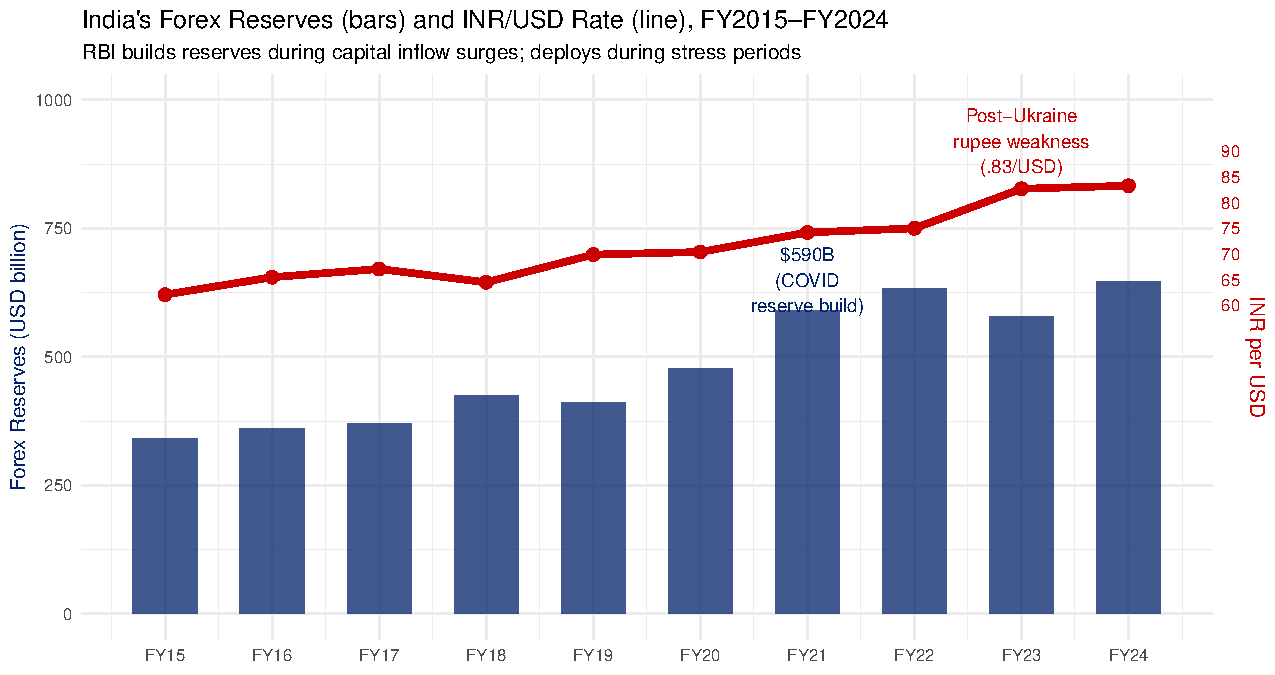
\includegraphics[keepaspectratio]{Lecture09_BoT_BoP_files/figure-beamer/fig-forex-reserves-1.pdf}}

}

\caption{India's Forex Reserves and INR/USD
Exchange Rate, FY2015--FY2024 Source: RBI, Database on Indian Economy
(DBIE).}
\label{fig-forex-reserves}

\end{figure}%
\end{frame}

\begin{frame}{Key Takeaways: Lecture 9}
\phantomsection\label{key-takeaways-lecture-9}
\textbf{1. National income identity:}
\(\text{CA} = Y - A = (S - I) + (T - G)\). A CA deficit means the
country borrows from abroad --- financed by FA inflows or reserve
drawdown.

\textbf{2. BoP accounting:}
\(\text{CA} + \text{KA} + \text{FA} + \Delta R = 0\). The BoP always
balances --- surpluses and deficits are in \emph{individual accounts},
not the overall BoP.

\textbf{3. India's external position (FY2024):} CA = -0.7\% GDP
(comfortable); remittances = \$120B (world's largest); services surplus
= \$163B; forex reserves = \$646B (11 months imports). External position
is \textbf{strong}.

\textbf{4. Marshall-Lerner condition:} \(|e_X| + |e_M| > 1\) must hold
for depreciation to improve TB. In the short run, M-L is typically NOT
satisfied → J-curve: TB worsens before improving.

\textbf{5. India 1991 crisis:} Reserves fell to \$1.2B (2 weeks
imports); India pledged 67 tonnes gold to the BoE. IMF bailout triggered
liberalisation --- delicensing, trade reform, FDI opening. Crisis →
structural reform.

\note{\textbf{6. Agricultural BoP:} India runs a trade surplus in
agriculture (\textasciitilde\$20B), but edible oil imports (-\$21B) are
the single largest structural weakness. MSP policy affects both food
security and export competitiveness.}
\end{frame}

\begin{frame}{Next Lecture Preview}
\phantomsection\label{next-lecture-preview}
\textbf{Lecture 10 --- Exchange Rates and Agricultural Trade} \emph{June
27, 2026}

\begin{itemize}
\tightlist
\item
  Fixed vs flexible exchange rate systems
\item
  Purchasing Power Parity (PPP): absolute and relative
\item
  Real exchange rate: \(q = eP^*/P\) and agricultural competitiveness
\item
  How rupee depreciation affects Indian rice and wheat exports
\item
  Dutch disease: can commodity booms harm agricultural exporters?
\end{itemize}

\note{\begin{itemize}
\tightlist
\item
  India's managed float: RBI intervention and the REER
\end{itemize}

\textbf{Preparation:} Review Salvatore Ch. 14--15 (Exchange Rates). Note
that India operates a \textbf{managed float} --- this means
understanding both PPP theory AND RBI's intervention behaviour. We will
use regression analysis of real exchange rate and export volume data.}
\end{frame}

\section{Appendix}\label{appendix}

\begin{frame}{Additional Resources}
\phantomsection\label{additional-resources}
\textbf{Further reading}

\begin{itemize}
\tightlist
\item
  Salvatore, \emph{International Economics} (relevant chapters)
\item
  Appleyard \& Field, \emph{International Economics} (relevant chapters)
\end{itemize}

\textbf{Key data sources}

\begin{itemize}
\tightlist
\item
  DGCI\&S: merchandise trade
\item
  RBI: balance of payments
\item
  APEDA: agricultural export statistics
\item
  WTO: tariff + trade databases
\end{itemize}
\end{frame}




\end{document}
